% !TEX root = ../main.tex
\chapter{National Income Accounting}
\label{ch:accounts}

Before we can explain why economies boom and slump, grow and stagnate, we need a way to measure what they produce. Macroeconomics is the study of aggregates --- total output, total income, total spending --- and an aggregate is only as useful as the number that stands for it. National income accounting is the system of definitions and identities that turns the sprawling activity of millions of households and firms into a handful of measured quantities. It is the macroeconomist's equivalent of a firm's financial statements: dull on its own, indispensable for everything that follows.

The central object is gross domestic product (GDP), the market value of everything an economy produces in a period. Most of this chapter is an extended unpacking of that one sentence, because almost every word in it is a deliberate choice with consequences. We then show that the same total can be reached three different ways --- by counting production, by counting income, or by counting expenditure --- and that the equality of these three routes is not a theorem to be proved but an identity built into the accounts. From the expenditure route we read off the famous decomposition of demand into consumption, investment, government purchases, and net exports; from the income route, the chain of refinements that runs down from GDP to disposable personal income; and from the financial market, the saving--investment identity that ties household thrift, the government deficit, and the trade balance together. We close with two practical matters: how output is sorted into industries, and how analysts guess at GDP between official releases.

A standing warning frames the whole enterprise. No single number summarizes an economy, and GDP in particular was designed to be \emph{measurable}, not to be a complete measure of welfare. Keeping straight what it does and does not count is half the battle.

\section{Gross Domestic Product}

\defn{Gross Domestic Product}{
\emph{Gross domestic product (GDP)} is the market value of all final goods and services produced within the geographic borders of an economy during a given period.
}

Read slowly, that definition contains five qualifiers, each of which excludes something. We take them one at a time.

\subsection{The Five Qualifiers}

\textbf{(1) A given period --- GDP is a flow.} GDP is always reported for a span of time, normally a quarter or a year; every country in the world publishes annual and quarterly figures. Because it is measured \emph{over an interval}, GDP is a \emph{flow}, not a \emph{stock}. A flow is a quantity measured per unit of time; a stock is a quantity measured at a point in time. The distinction is not pedantry --- it is the single most common source of confusion in macroeconomics, and one should form the habit of asking of every macro variable whether it is a stock or a flow.

Wealth, for instance, is a stock: at this instant the economy holds a definite total of assets. GDP is a flow, and the two are not the same thing. When Chinese GDP overtook Japanese GDP around 2010, it meant only that from that year onward China produced more goods and services each year than Japan did; it did not mean that China's accumulated \emph{wealth} had overtaken Japan's, which very plausibly had not.

\rmkb[Income versus wealth, and why finance nets out]{It helps to keep three related flows and stocks apart. \emph{Income} (a flow) is labor income --- wages, bonuses --- plus capital income --- returns \emph{on} assets, such as dividends and interest, but \emph{not} the capital stock itself. \emph{Wealth} (a stock) is the sum of real assets and financial assets. Macroeconomics is principally about income; wealth is more the concern of the individual. Note too that financial assets are not net wealth for society as a whole: every financial asset is some agent's claim on another agent, and summed across the economy these claims cancel. This is why macro accounting can ignore them and still add up.}

\rmkb[When monthly GDP appears]{There is normally no monthly GDP, because the data cannot be cleaned in time. But in special circumstances the authorities estimate it: during the 2022 pandemic disruptions in China, monthly figures were tracked closely to set growth targets and steady expectations --- roughly $-2.2\%$ in April, $-0.1\%$ in May, and $+4\%$ in June 2022, summing to about $+0.5\%$ for the second quarter. In China, a preliminary income-method estimate is released around the 16th--20th of the month; monthly real-economy data are largely \emph{nominal}, since there is no time to deflate them. The full expenditure-method annual accounts, which include the shares of household and government consumption, appear the following May or June.}

\textbf{(2) Market value.} Because GDP adds up apples and haircuts and software, it must value everything in a common unit, and that unit is the market price. The reliance on market prices has an immediate corollary: things that are never traded in a market have no observed price and so are, in principle, hard to count --- subsistence production, household chores, and illegal transactions among them. What matters is that the good or service \emph{can and does} change hands at a market price, not that a transaction has literally occurred for each unit (inventories, discussed below, are produced output that is counted before it is sold).

\textbf{(3) Geographic scope --- ``domestic.''} GDP is defined by \emph{territory}. China's GDP covers production within China's borders, whether the producer is a Chinese national or a foreigner. This is the natural choice in a globalized economy and matches the way local policy is tied to local conditions; we contrast it with the national measure (GNP) below.

\textbf{(4) Final, not intermediate, goods.} Whether a good is \emph{final} or \emph{intermediate} depends on its use. A good or service used up as an input into further production is an intermediate good; a final good is one bought for consumption or investment. GDP counts only final goods. The reason is to avoid \emph{double counting}: if we added the flour and the cake, the flour would be counted twice. Note that the very same physical good can be either, depending on use --- flour bought by a household to bake a cake at home is a final good, while flour bought by a bakery to bake cakes for sale is an intermediate good.

\textbf{(5) Marketed or imputed production.} GDP counts what is produced and sold at market, plus a few things that are not literally sold but \emph{should} be valued as if they were, by imputation. The leading example is the housing services that owner-occupiers ``buy'' from themselves: an imputed rent is added to GDP. (There is no contradiction between counting the purchase price of a house and counting the flow of housing services it later yields --- they are different things, as we explain under investment.)

\subsection{What Counts and What Does Not}

The five qualifiers settle most cases, but the boundary is fiddly enough that it is worth collecting the standard rulings in one place. The organizing principle is simple: \emph{GDP counts newly created value, once.}

\rmkb[Edge cases in what GDP counts]{
\begin{itemize}
    \item \emph{Nothing newly created, nothing counted.} Government taxes and transfer payments are not in GDP --- they merely redistribute existing funds. (The \emph{wages} of government employees \emph{are} in GDP, as payment for services produced.) Stock trades are not in GDP, being transfers of ownership with no new output; the stamp duty on a trade is not in GDP, being a transfer to the government; but a \emph{commission} is in GDP, because brokerage is a service produced.
    \item \emph{Only the newly created part.} The full sale price of a new house is not all GDP, because part of it is the value of the land. Only the value of the newly constructed building counts. The taxes paid to the government on purchase do not count.
    \item \emph{Inventories count as investment.} Goods produced this year but not yet sold are this year's output, whenever they eventually trade. In expenditure terms, when an inventory good is later sold, consumption (or investment) spending rises while the inventory falls by the same amount, and the two offset.
    \item \emph{Imputed values.} Output not sold in a market but conceptually marketable is imputed and counted --- owner-occupied housing services being the standard case.
    \item \emph{R\&D is now investment.} Research and development spending, once treated as an intermediate input to production, is now counted as investment.
    \item \emph{Services are valued at price, not quality.} A service enters at its price regardless of how good it was.
    \item \emph{Defensive expenditure inflates GDP.} Activity that merely offsets a negative externality is still counted, which overstates true output and welfare. If a firm pollutes while producing, its output adds to GDP, and the later cleanup adds to GDP again --- GDP is inflated twice over.
\end{itemize}
}

The last point is the sharpest reminder that GDP is a production tally, not a welfare index. The definition was chosen partly for its meaning and partly for its measurability, and as a result it deliberately leaves a great deal of value uncounted.

\subsection{From Domestic to National: GNP and GNI}

The geographic qualifier has a natural cousin. Where GDP draws its boundary around a \emph{territory}, gross national product draws it around a \emph{people}.

\defn{Gross National Product}{
\emph{Gross national product (GNP)} is the market value of all final goods and services produced by the \emph{nationals} of a country during a given period, wherever in the world they produce them.
}

The two measures differ only in who is included, and they are linked by a clean adjustment:
\[
\mathrm{GNP} = \mathrm{GDP} + \pr{\text{production by nationals abroad}} - \pr{\text{production by foreigners at home}}.
\]
For a large economy the gap between GDP and GNP is small. The World Bank uses per-capita GNP --- now reported as gross national income (GNI) --- to gauge how rich a country's people are, classifying economies as low-, middle-, or high-income; China is currently in the upper-middle-income band.

\section{The Circular Flow and the Fundamental Identity}

Why should the various ways of measuring output give the same answer? The reason is that one agent's expenditure is another agent's income, and the economy's payments chase each other around a closed loop. That loop is the \emph{circular flow}, sketched in Figure~\ref{fig:macro-1}.

\begin{figure}[h]
\centering
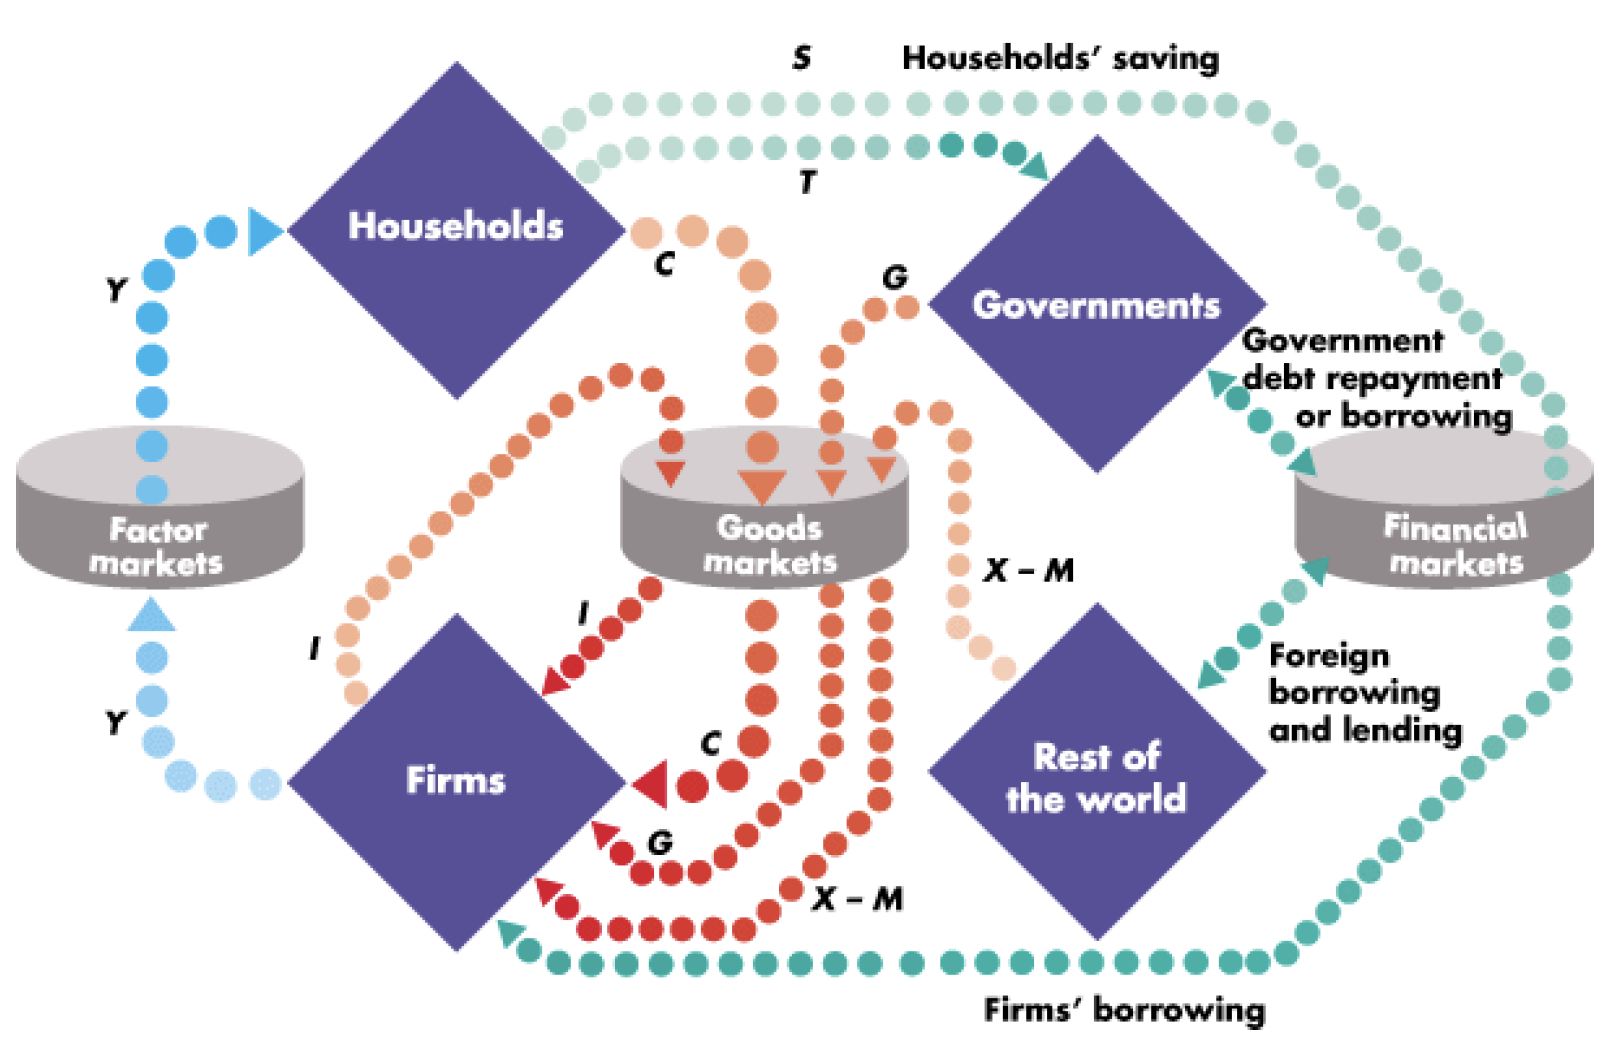
\includegraphics[width=\linewidth]{figures/fig1.png}
\caption{The circular flow of income: households, firms, the government, and the rest of the world transact across the goods market, the factor market, and the financial market, so that aggregate income equals aggregate expenditure.}
\label{fig:macro-1}
\end{figure}

The analysis centers on the \emph{household}. Households are the hinge of the whole system because they are responsible both for income and for spending: broadly, the household is the supplier on the factor market and the demander on the goods market. Income flows to households and is then split among consumption $C$, saving $S$, and taxes $T$, ultimately reappearing as the demands $C$, $I$, $G$, and net exports.

Three markets organize the picture. The \emph{goods market} links the main macroeconomic agents --- firms, households, the government, and the rest of the world. Firms supply this market; the demand comes from households, the government, and abroad. The \emph{factor market} closes the loop: the revenue firms earn on the goods market must flow back to pay the factors of production, and the suppliers of those factors --- earning the corresponding income --- are the households. The \emph{financial market} ties saving to investment, lets the economy lend to foreigners so that net exports can occur, and is closely bound up with the government's finances as well.

Because income and expenditure are the same payments seen from two sides, aggregate income (AI) equals aggregate expenditure (AE):
\begin{equation}
\mathrm{AI} = Y = C + I + G + \pr{X - M} = \mathrm{AE}.
\label{eq:macro-identity}
\end{equation}
The identity \eqref{eq:macro-identity} holds \emph{ex post}: realized income equals realized expenditure by construction. Aggregate demand is the \emph{ex ante} notion --- the planned, intended spending built up from desired $C + I + G + \mathrm{NX}$ --- and short-run fluctuations arise precisely when planned demand differs from realized output. The decomposition $C + I + G + \mathrm{NX} = \mathrm{AD}$ is therefore a short-run object, constantly fluctuating, and its components are sorted by the \emph{agent} doing the spending.

\subsection{The Three Drivers of Growth}

Sorting spending by agent runs into trouble in an economy like China's, where the state invests heavily and ownership is often blurred --- many state-owned enterprises operate under mixed or even private ownership, so it is frequently impossible to say whether a given outlay is public or private. The fix is to sort government spending $G$ not by \emph{who} spends but by the \emph{nature} of the spending, reassigning each piece of $G$ to either consumption or investment. Government \emph{consumption} folds into $C$, government \emph{investment} into $I$. (In principle $I$ then splits into private and public investment, but the statistics cannot separate them.) Sorting by nature collapses \eqref{eq:macro-identity} into
\begin{equation}
\mathrm{GDP} = C + I + \mathrm{NX}.
\label{eq:macro-three-drivers}
\end{equation}
These three terms are the celebrated ``three horses'' pulling growth: final consumption expenditure $C$, gross capital formation $I$, and net exports of goods and services $\mathrm{NX} = X - M$. The first two together, $C + I$, are \emph{domestic demand}; net exports are \emph{external demand}; and one can compute the contribution of each to a year's growth.

\section{Three Routes to the Same Total}

Equation~\eqref{eq:macro-identity} already hints that output can be counted in more than one way. There are three standard methods, and by construction they all arrive at the same GDP.

\subsection{The Production (Value-Added) Method}

\defn{Value Added}{
A firm's \emph{value added} is its sales revenue minus its spending on intermediate inputs (raw materials). GDP by the production method is the sum of value added across all productive units in the economy.
}

This method is the most direct unpacking of the definition: value added is exactly the new value a firm creates, and summing it avoids double counting the intermediate goods that passed through. Sales, intermediate purchases, value added, and GDP are all flows.

A subtlety worth stressing: the amount subtracted is \emph{only} intermediate-input cost, \emph{not} financial costs, labor costs, or selling costs such as wages and interest. The production method looks at \emph{production} --- the value created by productive units. In effect it treats productive units as the source of GDP and does not separately count the value households create by supplying factors; it captures the social production process as a whole. By contrast, summing \emph{all} sales across the economy yields gross industrial-and-agricultural output, in which intermediate sales are double-counted; a value-added tax, as levied in China, strips that double counting out.

\subsection{The Income Method}

\defn{The Income Method}{
GDP by the \emph{income method} is the sum of incomes earned by all agents in the economy, since value added accrues as income to someone.
}

The incomes that sum to GDP are wage income, interest income (the return on working capital), tax income, and \emph{accounting} profit --- where accounting profit includes both economic profit and \emph{rent}. The rent term captures the fact that machinery and equipment used in one's own production could instead have been rented out on the market; using it oneself is, in effect, producing and consuming the rental service. Inventories enter here too, understood as value created this year that earns its return next year.

\subsection{The Expenditure Method}

\defn{The Expenditure Method}{
GDP by the \emph{expenditure method} is the sum of spending on final goods and services: $C + I + G + (X-M)$.
}

The focus is the goods market. Set the government and trade aside for a moment: every final good on the goods market is bought either by a household or by a firm. Machinery and equipment bought by firms as capital goods are investment spending $I$; almost everything else is household consumption spending $C$ --- with the standard exception that a house purchase counts as investment, not consumption. Reintroducing the government and trade changes nothing essential; the focus stays on the goods market. By convention, goods bought by households --- housing aside --- are counted entirely in the period of purchase.

\state{Three methods, one number}{
Production, income, and expenditure are three vantage points on the same circular flow. The value added in production accrues as income, and that income is spent. The three methods therefore measure the same GDP, and their equality is an accounting identity, not an empirical finding.
}

\section{Financial-Market Accounting and the Saving--Investment Identity}

The financial market connects the same four agents --- households, the government, firms, and foreigners. Household \emph{saving} $S$ is the chief source of funds; firms draw on those funds to finance investment $I$; the government, when it runs a deficit $(G-T)$, must borrow from the market; and foreigners, when they buy the country's net exports $(X-M)$, must borrow as well. Following the GDP-accounting logic, treat saving $S$ as the total ``income'' supplied to the financial market and $I + (G-T) + (X-M)$ as the total ``use'' of those funds.

We can derive the relationship cleanly. Income is used in exactly three ways --- consumption, saving, and taxes --- which is the financial-flow identity
\begin{equation}
Y = C + S + T.
\label{eq:macro-uses}
\end{equation}
Setting the uses of income \eqref{eq:macro-uses} equal to the expenditure identity $Y = C + I + G + (X-M)$ and cancelling $C$ gives $S + T = I + G + (X-M)$, that is,
\begin{equation}
S = I + \pr{G - T} + \pr{X - M}.
\label{eq:macro-saving}
\end{equation}
This matches the intuition above: saving funds private investment, plus the government's deficit, plus foreigners' net borrowing to buy our exports. Solving instead for investment,
\begin{equation}
I = S + \pr{T - G} + \pr{M - X}.
\label{eq:macro-investment}
\end{equation}
Investment thus draws on three pools of funds:
\begin{itemize}
    \item private saving, $S$;
    \item the government's budget surplus, $T - G$;
    \item net borrowing from foreigners, $M - X$.
\end{itemize}
Here $S$ alone is \emph{private saving}, and $S + (T-G)$ is \emph{national saving}.

\rmkb[Reading the signs]{Two of the terms in \eqref{eq:macro-investment} flip sign relative to \eqref{eq:macro-saving}, and it is worth seeing why. Taxes $T$ are redistribution --- a second round of allocation following a fairness principle, as with a progressive income tax. (Note that Chinese taxation is essentially a tax on wages, not on property.) The term $T-G$ says that the government raises funds by taxation and spends on the goods market; a surplus is released \emph{into} the financial market, while a deficit is borrowed \emph{from} it. The term $M-X$ says that when foreigners buy our net exports they must pay in our currency, which they obtain by borrowing from us, draining funds from the domestic financial market; hence $M-X = -(X-M)$, the mirror image of the foreign borrowing that appears in \eqref{eq:macro-saving}.}

\rmkb[Saving in the macro sense]{Three cautions on saving. First, \emph{national saving} is total income minus total consumption, and China's national saving rate is far higher than most countries'; saving and investment are very strongly positively correlated. Second, saving in the macro sense is not the everyday notion of putting money aside --- it is funds that enter and circulate through the financial market. Third, foreign direct investment brings, more than money, advanced technology and management know-how.}

\section{Investment and Capital Formation}

Among the three drivers, investment is the one most easily misunderstood, so it deserves its own treatment. The measured counterpart of investment in the accounts is \emph{gross capital formation}, and its job is to track changes in the economy's stock of real capital.

\defn{Capital Law of Motion}{
Capital is a stock that depreciates and is replenished by the flow of investment. Writing $K_t$ for the capital stock, $I_t$ for gross investment, and $\delta$ for the depreciation rate,
\[
\Delta K = K_2 - K_1 = I_1 - \delta K_1,
\qquad\text{equivalently}\qquad
K_2 = \pr{1-\delta} K_1 + I_1.
\]
}

This is investment in the true sense, and it has two components: gross fixed capital formation and the change in inventories (the latter a small share of the total). The distinction between investment and mere asset trading is essential. Apart from the change in inventories, only outlays that \emph{form capital} --- meaning physical, real capital --- are investment in the macroeconomic sense. Buying a share of stock, by contrast, transfers ownership of a financial asset; the asset's price may change in the process, but no new capital good is produced.

\rmkb[Fixed-asset investment versus capital formation]{Two related statistics should not be confused. \emph{Fixed-asset investment}, an accounting category, includes spending on land, on used equipment, and on used buildings --- but these are \emph{not} in gross capital formation, since they do not create new capital. Below-scale projects, and intangible investments such as computer software, are also excluded. Land-purchase fees (from land auctions) are in fact a primary revenue source for local governments. As a result the gap between reported fixed-asset investment and gross capital formation is large. Cross-province fixed-asset investment, moreover, can be double-counted, so the provincial figures can sum to \emph{more} than the national total. China's statistical bureau publishes fixed-asset investment as a cumulative year-to-date figure, since single-month values swing wildly; investment data are harder to collect than consumption data and involve much messier computation, and the January and February figures are reported jointly to absorb the timing of the Spring Festival. The three most important sub-indicators of fixed-asset investment are real estate, infrastructure, and manufacturing.}

\rmkb[Housing is always investment]{Any house purchase, of any type, counts as investment, never as consumption --- the holding period is long enough and the sum large enough that it has investment character. This matters for the macroeconomy: new-home sales in China have lately fallen by more than 20\%, and the broader weakness of the economy is tightly linked to the real-estate downturn.}

It is convenient at this point to fix some factor-price notation we will reuse. Let $r$ denote the \emph{capital rental price}, which is \emph{not} the same concept as the interest rate, and let $w$ denote the labor rental price (the wage). Output is produced from capital and labor through a production function $Y = F(K, L)$. The deeper contrast between raw materials and capital is one of durability: raw materials are consumed in one shot, whereas capital is a durable good whose ``consumption'' is precisely depreciation, and whose replenishment runs through the process of investment. Human capital shares this attribute --- it too depreciates with the passage of time.

\section{From GDP to Disposable Income}

GDP is a \emph{gross} measure: it includes the part of output that merely replaces capital worn out during the year. By the same token, gross investment $I$ includes the part spent replacing depreciated capital. To move from the gross production total toward what people actually have to spend, we peel off depreciation and then make a series of further adjustments. The chain is mechanical but worth having in one place.

\defn{From GDP down to Disposable Personal Income}{
\[
\ba
\mathrm{NNP} &= \mathrm{GDP} - \text{depreciation},\\
\text{National Income} &= \mathrm{NNP} - \text{indirect business taxes},\\
\text{Personal Income} &= \text{National Income} - \text{corporate profits} - \text{net interest}\\
&\quad {} + \text{dividends} + \text{government transfers} + \text{personal interest income},\\
\text{Disposable Personal Income} &= \text{Personal Income} - \text{personal taxes}.
\ea
\]
}

Net national product (NNP) strips depreciation out of the gross total; subtracting indirect business taxes gives national income, the total earned by factors of production; personal income adjusts national income for the income that is earned but not received (corporate retained earnings and net interest) and for the income received but not earned in production (transfers, dividends, personal interest); and removing personal taxes leaves disposable personal income, the amount households are free to consume or save.

\section{The Government Budget and Fiscal Goals}

The government's accounts enter the circular flow through taxes raised and purchases made, and the difference between the two is the budget balance.

\defn{Government Budget Balance}{
\[
\text{Government Budget Balance} = T - G,
\]
the excess of tax revenue $T$ over government spending $G$; it is a surplus when positive and a deficit when negative.
}

Fiscal policy can be pointed at two quite different goals. The first is a \emph{balanced-budget} strategy --- living within one's means, keeping $T-G$ at zero. The second takes \emph{economic growth} as the central purpose of fiscal policy, accepting deficits when they serve growth.

\rmkb[State capacity and China's fiscal conservatism]{Which goal a state can pursue depends on its fiscal capacity, and history is instructive. England's Glorious Revolution and Bill of Rights sharply raised the state's ability to tax and borrow, helping clear the path for the Industrial Revolution. Late-imperial China, despite a more absolute concentration of power, taxed weakly and laid only a light per-capita burden, so its fiscal capacity --- and therefore its military and defensive strength --- was correspondingly weak. The modern Chinese state still carries something of that legacy: it keeps tight control over the deficit ratio and prefers debt as low as possible, a conservative fiscal tradition. Yet today's downward pressures make the ancient balanced-budget instinct ill-suited to circumstances; the appropriate strategy now is growth, not balance. China's reported ratio of fiscal activity to GDP is modest, but its \emph{hidden} liabilities are large.}

\section{The Industrial Composition of GDP}

Total output can be sorted not only by who spends it but by where it is produced. The standard partition is into three sectors.

\defn{The Three Sectors}{
\begin{itemize}
    \item The \emph{primary sector} comprises agriculture, forestry, animal husbandry, and fishing.
    \item The \emph{secondary sector} comprises industry and construction.
    \item The \emph{tertiary sector} is services.
\end{itemize}
}

\rmkb[Sector conventions and structural change]{Several practical notes. China classifies the \emph{services} within agriculture, forestry, animal husbandry, and fishing as part of the primary sector, so the tertiary sector differs slightly from ``services'' as such, though the two are numerically close; agricultural goods cannot be used to balance trade. ``Industry'' within the secondary sector covers three broad categories: mining, manufacturing, and the production and supply of electricity, heat, gas, and water. Sector shares are usually read both as a share of GDP and as a share of total employment, and their movement is used to gauge a country's structural transformation. China's fastest-growing sector today is the tertiary, at roughly 60\% of the economy.}

A word of caution about reading these shares as policy targets. Structural change should be understood as a \emph{result}, not a \emph{cause}. One cannot copy another country's admired sector mix onto one's own economy and expect to copy its success. Manufacturing remains a powerful engine of growth; even if a larger service share is desirable, what is needed is \emph{better} manufacturing, not \emph{less} of it --- just as the answer to environmental problems is not a romantic retreat to a pastoral economy and a single-minded cut in carbon, but rapid growth that lets the economy reduce carbon as it advances.

\rmkb[Consumption rate up, investment rate down]{China is now a consumption-driven economy: its consumption rate has risen and its investment rate has fallen. The temptation, when short-run growth disappoints, is to blame weak consumption and to stimulate it. But the lesson of reading structure as a result rather than a cause cuts the other way. Rapid growth has historically rested on rapid \emph{investment}, not rapid consumption. China's investment rate is in fact far higher than America's (on the order of 40\% versus 16\%), and the claim that China over-invests is overstated: the problem is not too much investment but investment in the wrong places --- investing \emph{badly}, not investing too much. Equally, the weakness of consumption is not a problem of consumption \emph{itself}: slowing consumption growth reflects problems with income and the social safety net, the main cause being a rapid decline in disposable income, and so cannot be cured by stimulating consumption alone.}

\section{Proxy Indicators for GDP}

GDP is in a sense a theoretical construct, computed and released with a lag. Between releases, analysts lean on faster real-world series as side indicators. Each carries useful signal and characteristic noise.

\begin{enumerate}
    \item \emph{Electricity consumption and freight volume.} Both track physical activity, but both depend on the \emph{structure} of the economy: it is entirely possible for electricity and freight growth to slow even as overall economic activity speeds up, if the activity shifts toward less energy- and transport-intensive sectors.
    \item \emph{New credit.} A monthly series, but tightly bound to the central bank's monetary policy, to macroprudential policy, and to the level of financial development; its movements need not reflect real activity at all.
    \item \emph{The purchasing managers' index (PMI).} A monthly, seasonally adjusted index, with 50\% as the dividing line between expansion and contraction. The PMI is the first comprehensive macro reading available each month. Its \emph{new-orders} component is a leading indicator that forecasts future production and correlates strongly with real-economy series; the central bank uses the PMI in its own forecasting.
    \item \emph{Retail sales of consumer goods.} Retail sales of physical goods plus food-and-beverage services. This is \emph{not} the same as consumption $C$ in the national accounts --- services such as travel and education are excluded --- but it is easier to collect, being gathered mainly from firms and merchants.
\end{enumerate}

\rmkb[What retail sales hide, and durables versus perishables]{The single most important item within retail sales is the automobile, much as pork dominates the consumer price index. Consumption splits into \emph{perishable goods} (one-off consumption) and \emph{durable goods}; the longest-lived, highest-value purchase is typically the car, within which new-energy vehicles are the main driver --- and which carry an element of investment. The pandemic sharply compressed the settings and means of consumption. Perishables and services cannot be deferred, but durable consumption can be postponed, sometimes producing compensatory spending later --- weddings (jewelry) and automobiles being the leading cases. (Hence the ``lipstick effect'': trading down to small luxuries in a downturn.)}
